\section{Frontend, dokumentasi interaktif, dan deployment}
\subsection{Frontend Ruang UMKM}
Frontend pada route \code{/} menghubungkan katalog, keranjang, pembuatan
pesanan, dan riwayat melalui gateway yang sama. Halaman menyediakan tiga
produk, perubahan quantity, total perkiraan, nama pemesan, serta input API
key untuk operasi pesanan. Harga akhir dan ketersediaan stok tetap
ditentukan service, bukan nilai yang ditampilkan klien.

\begin{figure}[H]
\centering
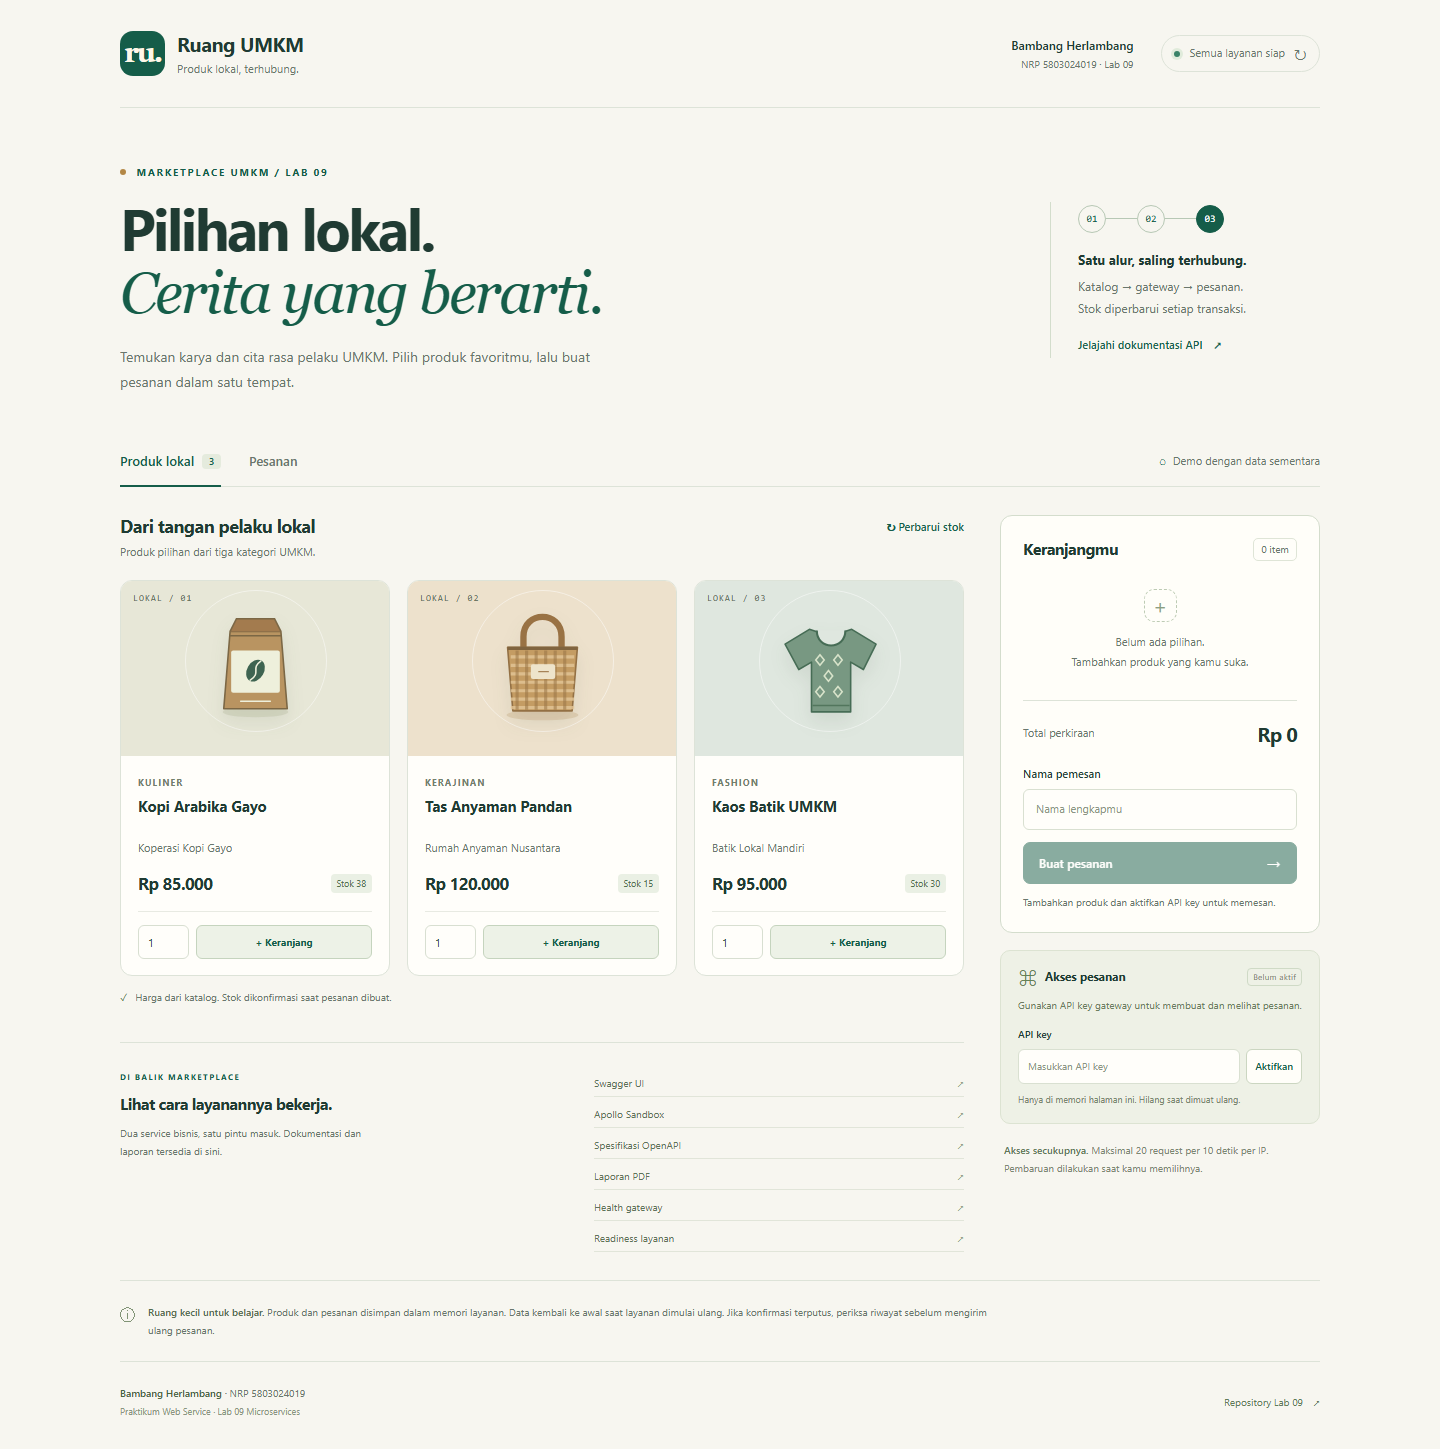
\includegraphics[width=\linewidth,height=.66\textheight,keepaspectratio]{frontend.png}
\caption{Frontend lokal Ruang UMKM: daftar produk, keranjang, dan akses
pesanan. Key belum diaktifkan pada tangkapan ini.}
\end{figure}

Tautan Swagger UI, Apollo Sandbox, OpenAPI JSON, laporan PDF, health, dan
readiness tersedia dari halaman. API key hanya disimpan dalam memori sesi
halaman; tidak ditulis ke localStorage atau sessionStorage.

\clearpage
\subsection{Checkout dan riwayat pesanan}
Pengujian browser lokal mencatat checkout dua kopi berhasil: stok yang
terbaca sebelum transaksi adalah 38 dan setelah transaksi 36. Pengujian
ini terpisah dari smoke test 40 menjadi 38 pada bagian sebelumnya.
Halaman riwayat menampilkan pesanan, rincian barang, harga, dan status.

\begin{figure}[H]
\centering
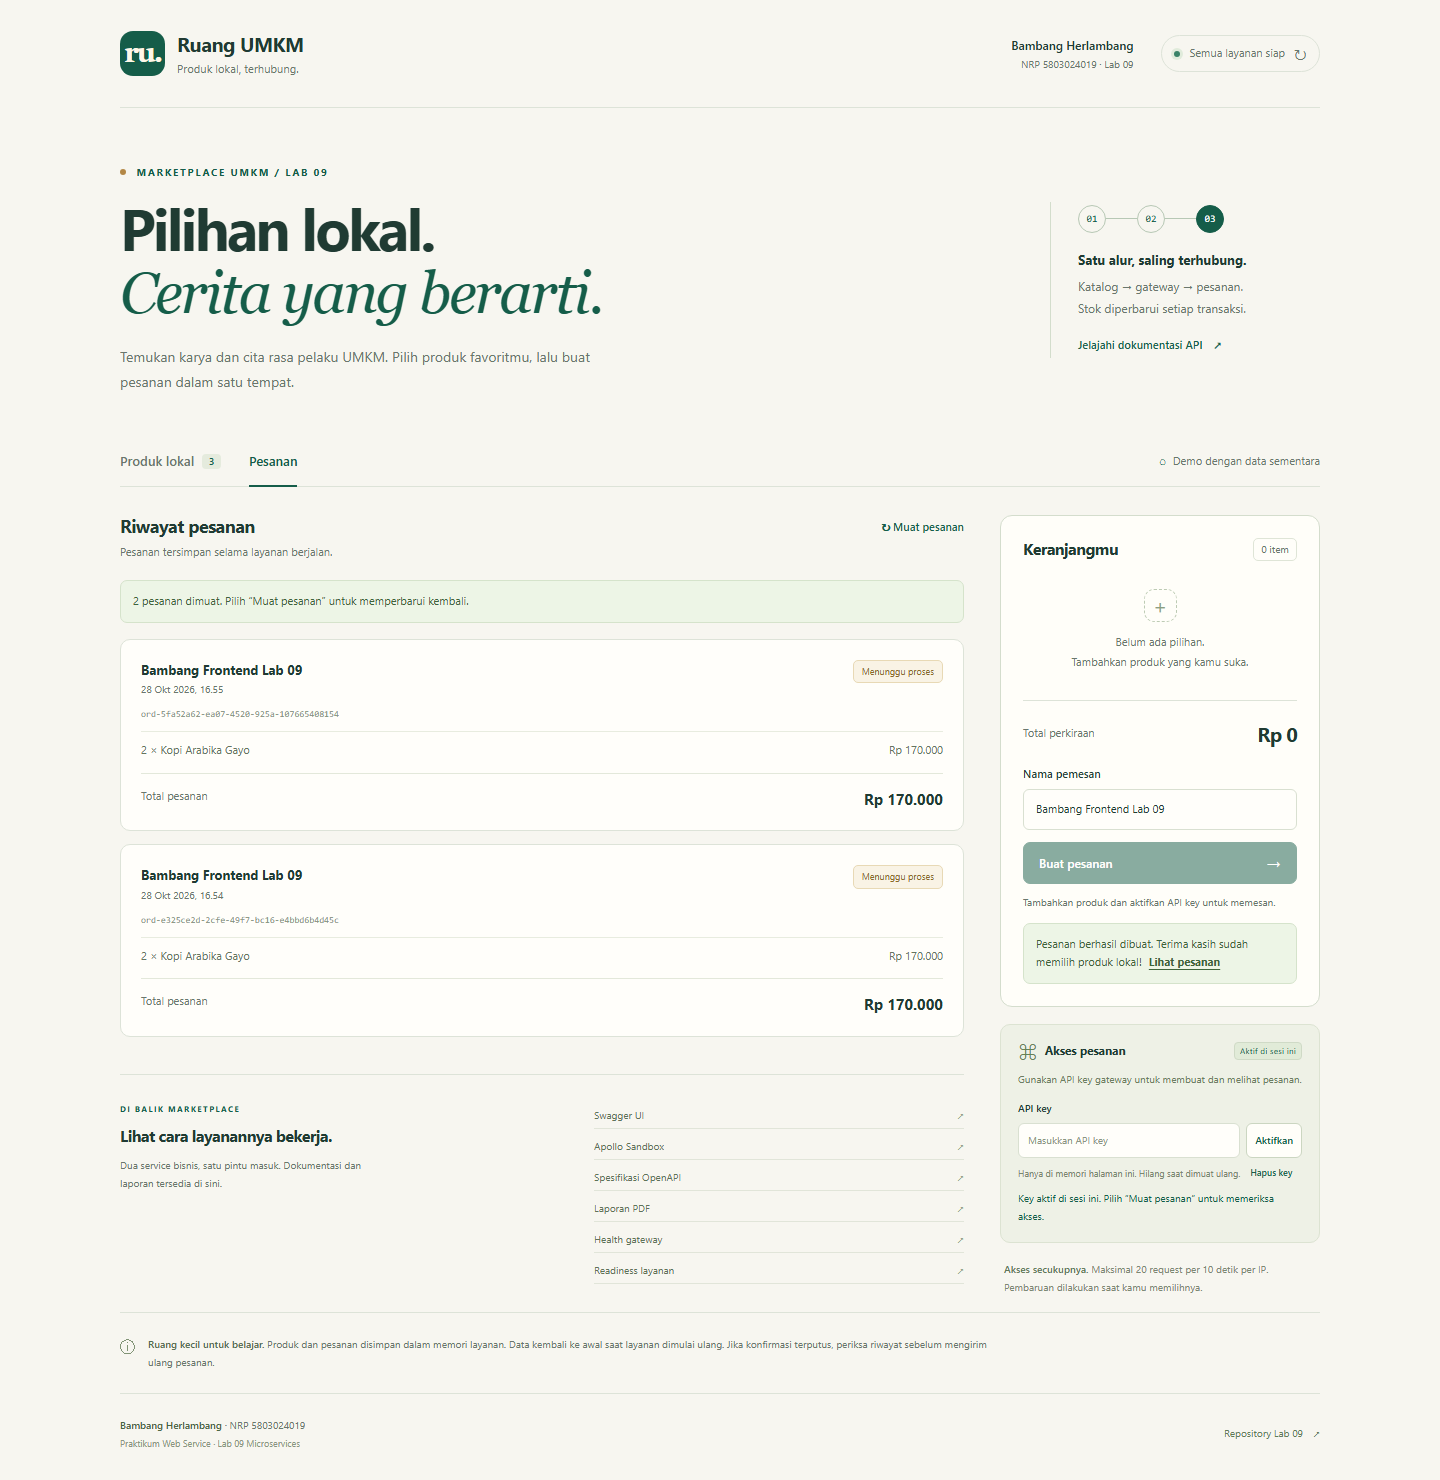
\includegraphics[width=\linewidth,height=.69\textheight,keepaspectratio]{frontend-orders.png}
\caption{Riwayat pesanan lokal setelah checkout melalui frontend. Nilai
key tidak ditampilkan; halaman menggunakan kredensial sesi sementara.}
\end{figure}

Rekaman \path{docs/evidence/ui/ui-verification.json} memuat hasil checkout,
penolakan API key salah, pengujian mobile, Swagger, dan pemuatan iframe
Apollo. Pengujian browser tersebut tidak mencatat page error.

\clearpage
\subsection{Tampilan mobile dan key tidak valid}
Pada viewport 390 piksel, verifikasi browser tidak menemukan overflow
horizontal. Produk, keranjang, form pesanan, dan navigasi disusun ulang
untuk layar sempit. Key salah ditolak dan halaman menampilkan pesan
kegagalan tanpa menyimpan nilai key dalam browser storage.

\begin{figure}[H]
\centering
\begin{minipage}[t]{.48\linewidth}
\centering
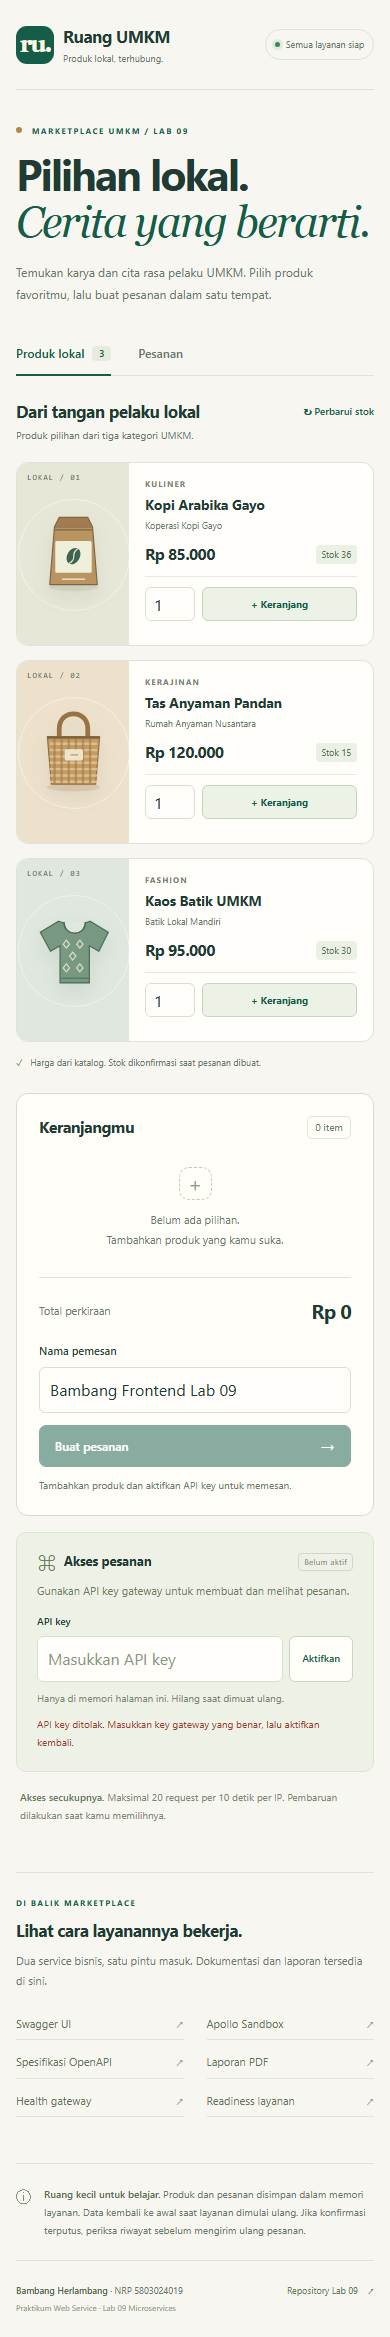
\includegraphics[width=.78\linewidth,height=.70\textheight,keepaspectratio,trim=0 1087bp 0 0,clip]{frontend-mobile.png}
\end{minipage}\hfill
\begin{minipage}[t]{.48\linewidth}
\centering
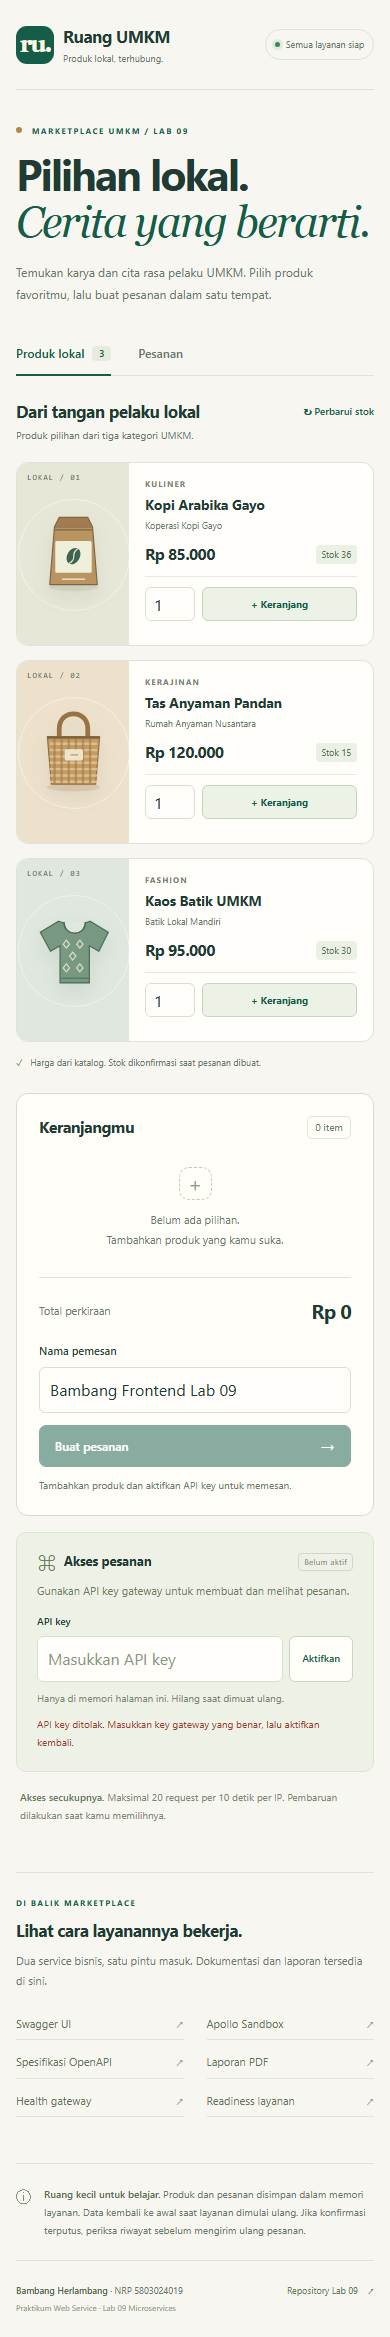
\includegraphics[width=.78\linewidth,height=.70\textheight,keepaspectratio,trim=0 0 0 1250bp,clip]{frontend-mobile.png}
\end{minipage}
\caption{Dua potongan berurutan dari satu screenshot mobile lokal:
katalog pada bagian atas dan form beserta pesan key ditolak pada bagian
bawah. Isi gambar tidak diubah.}
\end{figure}

\clearpage
\subsection{Swagger UI dan spesifikasi OpenAPI}
Swagger UI tersedia pada \code{/docs/} dan memuat spesifikasi
\code{/openapi.json}. Dokumentasi meliputi endpoint katalog, pesanan,
reservasi, GraphQL, health, serta respons error. Fungsi \textit{Authorize}
memungkinkan key dikirim untuk operasi yang memerlukannya tanpa
menanamkan nilai key dalam spesifikasi.

\begin{figure}[H]
\centering
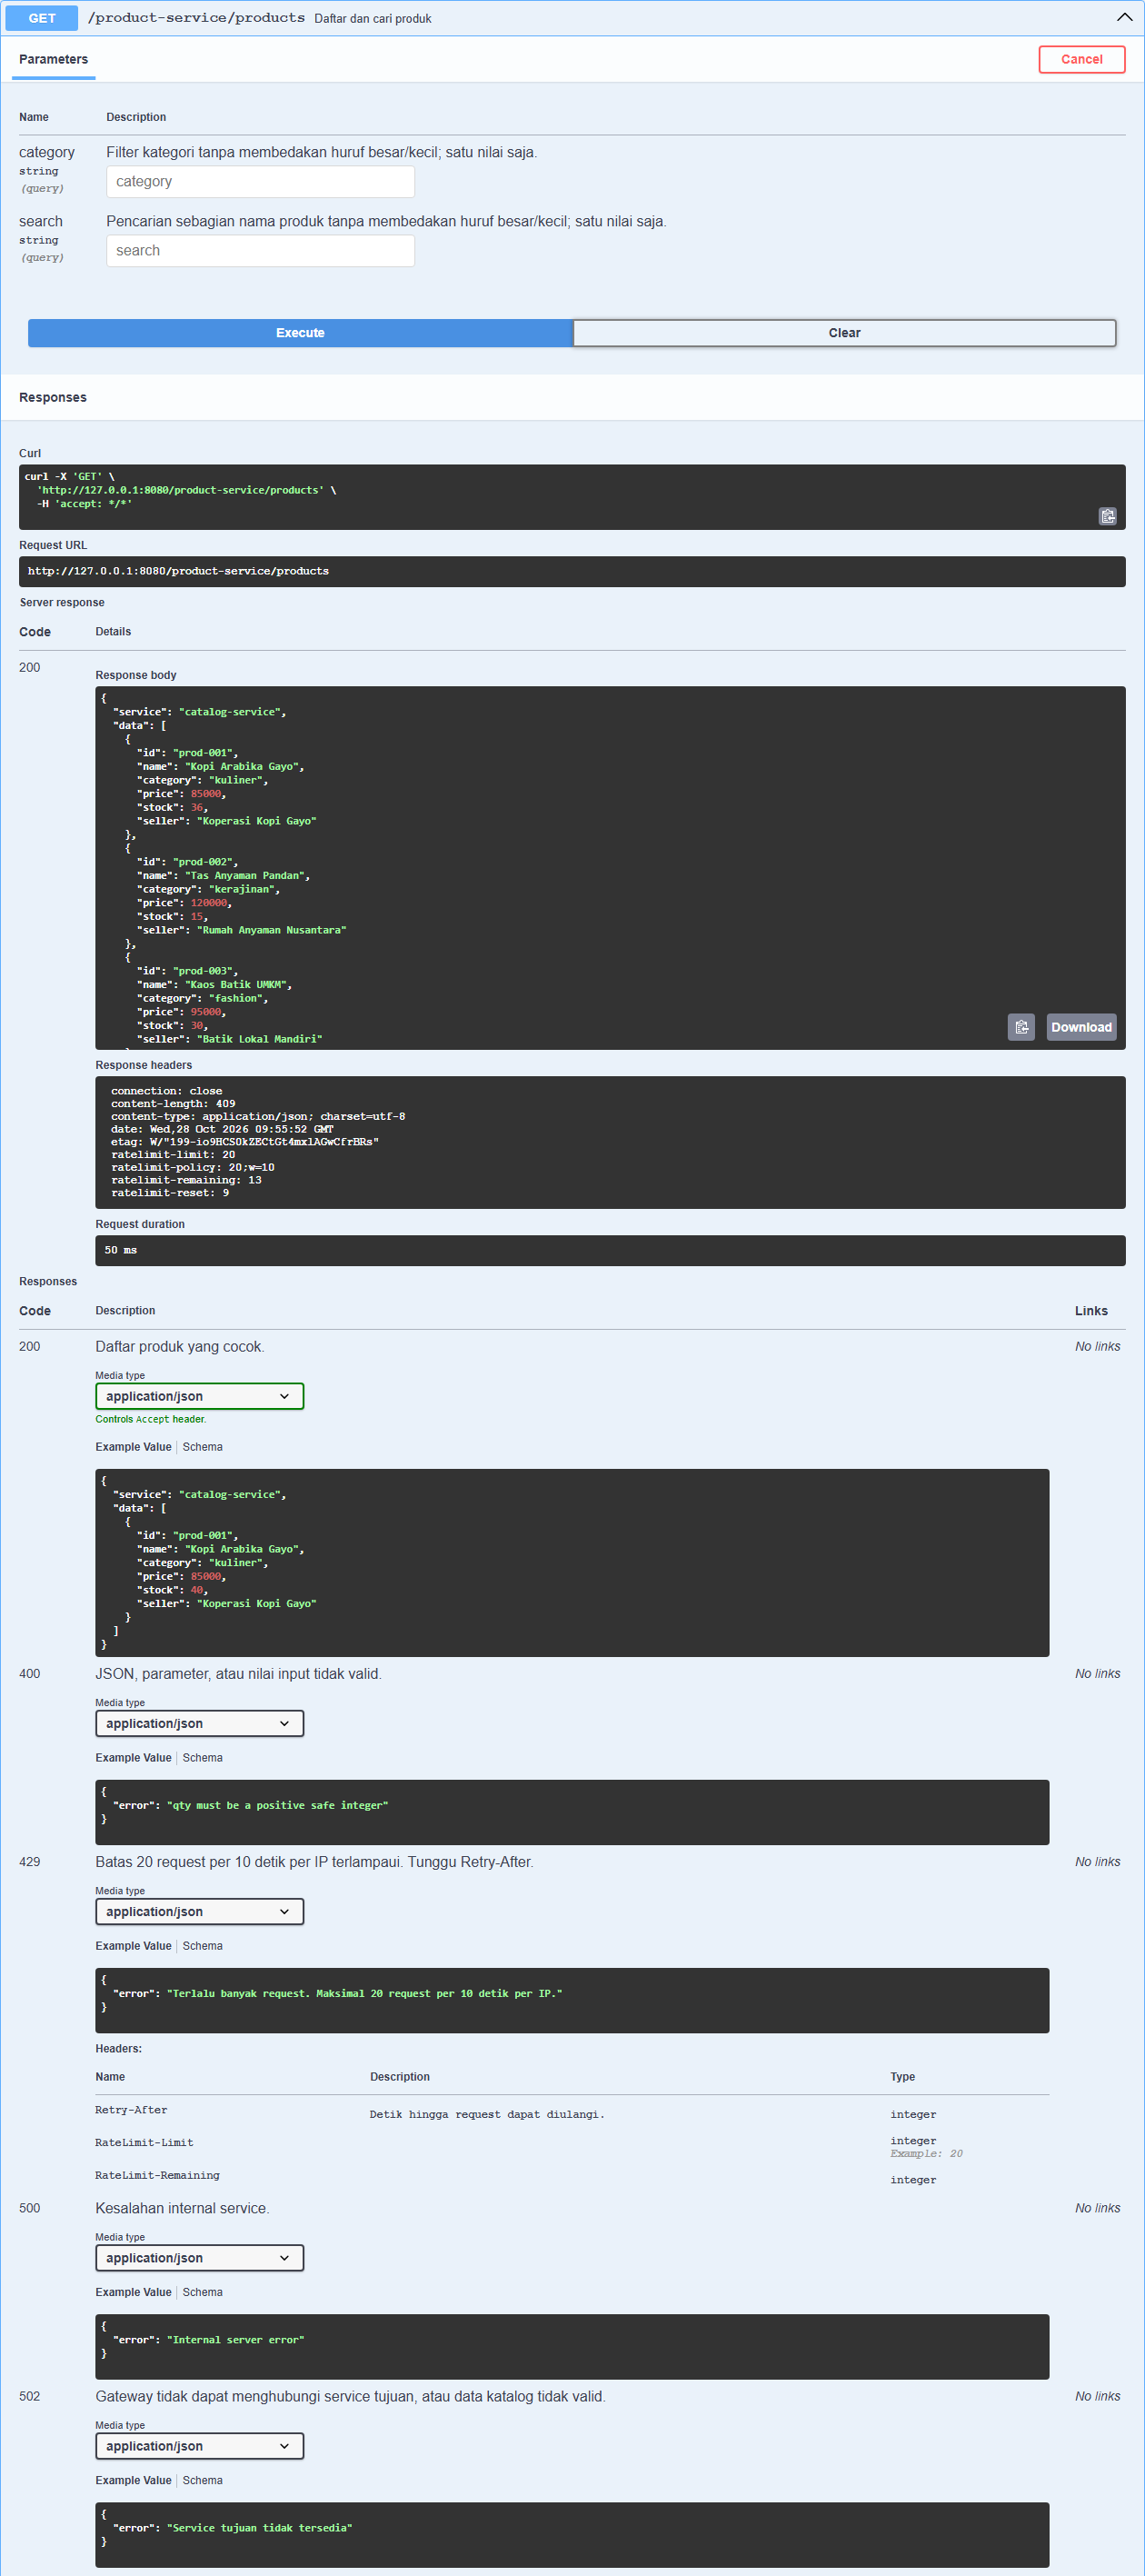
\includegraphics[width=\linewidth,height=.72\textheight,keepaspectratio,trim=0 1400bp 0 0,clip]{swagger-response.png}
\caption{Swagger Try it out pada gateway lokal mengembalikan HTTP 200
dan daftar produk. Area respons aktual ditampilkan; contoh respons statis
di bawahnya dipotong agar tidak tertukar sebagai bukti eksekusi.}
\end{figure}

Halaman dokumentasi tidak memakai kuota request API. Request yang dibuat
melalui Try it out tetap melewati route gateway, pemeriksaan key, dan
rate limit yang sama dengan klien lain.

\clearpage
\subsection{Apollo Sandbox dan GraphQL katalog}
Apollo Sandbox tersedia pada \code{/sandbox}. Endpoint GraphQL gateway:
\path{/product-service/graphql}. Halaman memakai Embedded Sandbox Apollo,
menyediakan query awal katalog, dan dapat membuka endpoint yang sama di
Apollo Studio. SDK tersebut memerlukan akses internet.

\begin{figure}[H]
\centering
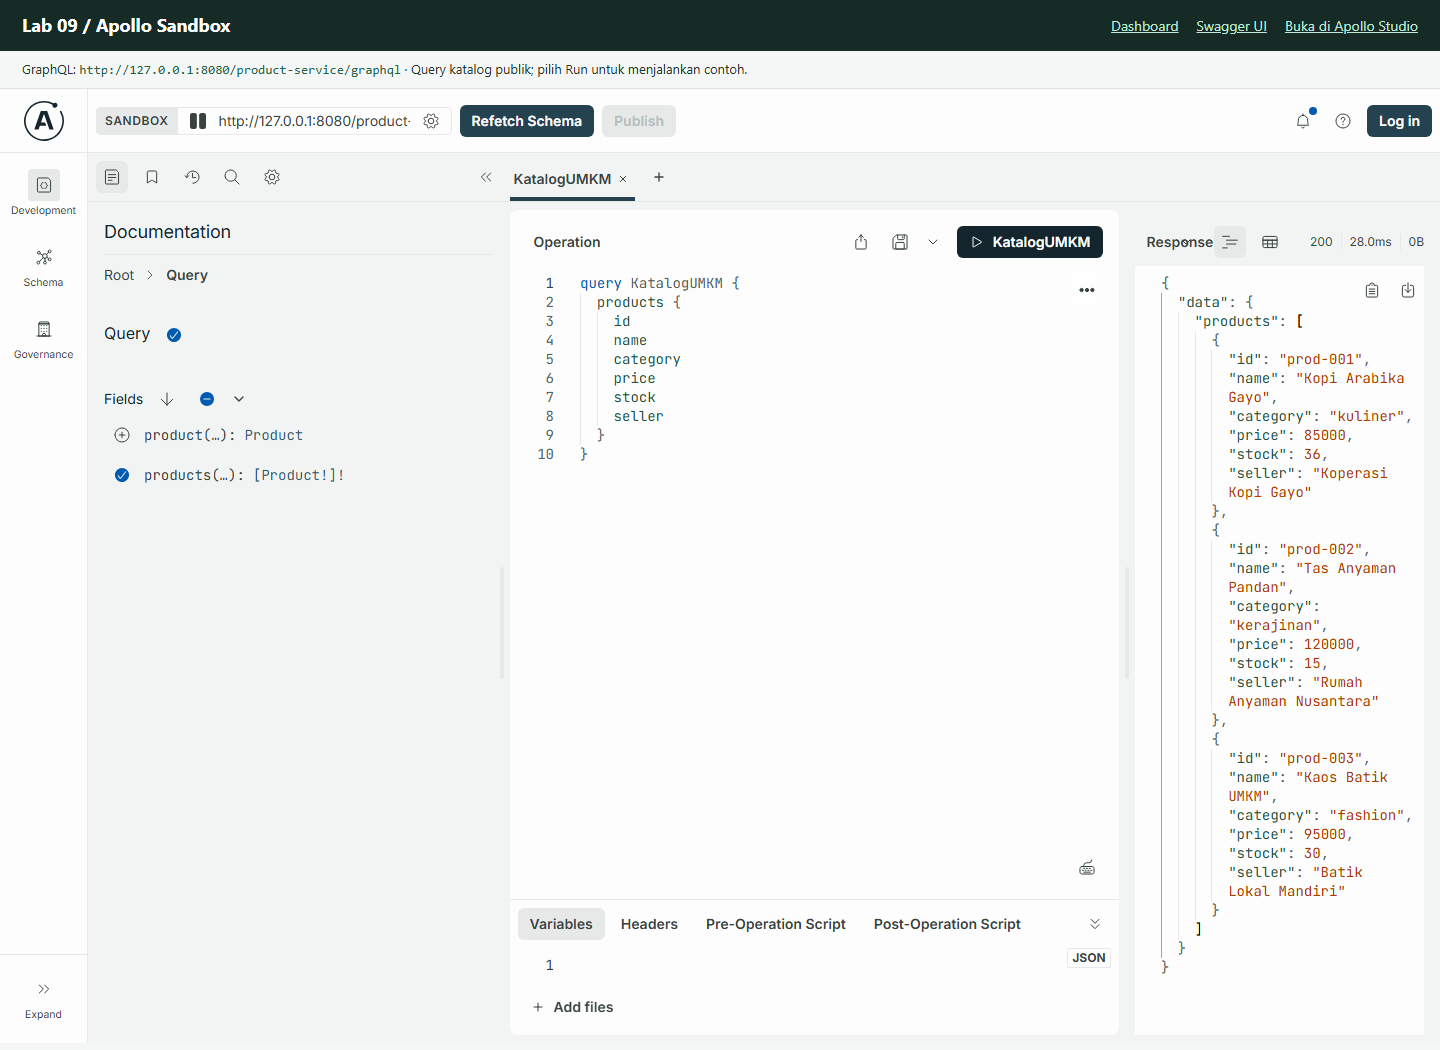
\includegraphics[width=\linewidth]{apollo-sandbox.png}
\caption{Operasi KatalogUMKM dijalankan melalui tombol Run pada Apollo
Sandbox lokal. Respons HTTP 200 menampilkan tiga produk beserta harga
dan stok; panel respons terlihat di sisi kanan.}
\end{figure}

\begin{lstlisting}
query KatalogUMKM {
  products { id name category price stock seller }
}
\end{lstlisting}
Hasil eksekusi tombol Run direkam dalam
\path{docs/evidence/ui/apollo-query.json}: status 200 dan tiga produk.
Query GraphQL katalog juga diverifikasi pada suite HTTP otomatis.
Berbagi akses lintas origin dibatasi pada endpoint GraphQL katalog yang
bersifat baca; kredensial pesanan tidak dibutuhkan untuk query tersebut.

\clearpage
\subsection{Konfigurasi deployment Render Free}
Deployment disiapkan pada \textbf{service Render terpisah khusus Lab 09},
menggunakan repository dan branch \code{main} Lab 09. Blueprint
\code{render.yaml} mendefinisikan satu instance Free yang menjalankan tiga
proses terpisah: gateway, katalog, dan pesanan. Hanya gateway yang
dipublikasikan; backend tetap pada loopback.

\begin{table}[H]
\small
\begin{tabularx}{\linewidth}{@{}L{3.7cm}Y@{}}
\toprule
Konfigurasi & Nilai \\
\midrule
Runtime / versi & Node.js 22 \\
Nama service & \code{prakwebservice-lab09-microservices} \\
Region / plan & Singapore / Free \\
Build & \code{npm ci --omit=dev} \\
Start & \code{npm start} \\
Health check & \code{/readyz} \\
Gateway & Host \code{0.0.0.0}, port dari platform, \code{TRUST_PROXY=1} \\
Backend & Host loopback; katalog port 3000, pesanan port 3001 \\
Key server & Digest SHA-256 melalui \code{API_KEY_SHA256} \\
\bottomrule
\end{tabularx}
\caption{Konfigurasi deployment pada blueprint Lab 09.}
\end{table}

\textbf{Status verifikasi publik.} Konfigurasi deployment Render Free
pada service terpisah telah disiapkan; verifikasi URL HTTPS, health,
frontend, Swagger, Apollo Sandbox, dan pesanan publik diperbarui setelah
layanan aktif. Bagian ini mencatat konfigurasi dan tidak menyatakan
deployment telah berhasil.

Collection Postman JSON dan environment lokal tersedia dalam
\path{docs/postman/}. Environment publik menggunakan base URL gateway
deployment, sementara nilai API key tetap diisi secara lokal oleh klien.
Data demo tetap bersifat in-memory pada deployment ini.
